
% DO NOT CHANGE THIS FILE.

% This file contains all the formatting information required
% to make your document fit the necessary style requirements.
% Any changes you make to this file will be over-written at
% the time of submission. If for any reason you feel it is
% necessary to make changes to this, such as a missing package,
% please contact the editors of North East Indian Linguistics
% to discuss the suggested changes.

% DO NOT MAKE ANY CHANGES WITHOUT APPROVAL FROM THE EDITORS.

\documentclass[12pt]{article}

% margins, paper size
\usepackage{geometry} 
\geometry{
	a4paper,
	bottom=2.5cm,
	left=2.5cm,
	right=2.5cm,
	top=2.5cm,
}

% trees
\usepackage{tikz}
\usetikzlibrary{trees, arrows}
\usepackage{tikz-qtree,tikz-qtree-compat}
\tikzstyle{level 1}=[level distance=2em, sibling distance=0.25cm]
\tikzstyle{level 2}=[level distance=2em, sibling distance=0.25cm]
\tikzstyle{level 3}=[level distance=2em, sibling distance=0.25cm]
\tikzstyle{level 4}=[level distance=2em, sibling distance=0.25cm]
\tikzstyle{level 5}=[level distance=2em, sibling distance=0.25cm]

% fonts
\usepackage{fontspec}
\newfontfamily\tgtermes{TeX Gyre Termes}
\setmainfont{Times New Roman}[
	ItalicFont={Times New Roman Italic},
	BoldFont={Times New Roman Bold}
]
\newfontfamily\tgtermes{TeX Gyre Termes} % small caps fallback
\makeatletter
  \begingroup
    \tgtermes
    \DeclareFontShape{\f@encoding}{\rmdefault}{m}{sc}{%
      <-> ssub * \f@family/m/sc}{}
    \DeclareFontShape{\f@encoding}{\rmdefault}{bx}{sc}{%
      <-> ssub * \f@family/bx/sc}{}
  \endgroup
\makeatother
\newfontfamily\oblique{Times New Roman Italic}

% bold captions at 10pt
\usepackage[small,font=bf,hang,labelsep=endash]{caption}

% font sizes
\makeatletter
\renewcommand\large{\@setfontsize\large{13pt}{15pt}}
\renewcommand\normalsize{\@setfontsize\normalsize{12pt}{14pt}}
\renewcommand\tiny{\@setfontsize\tiny{8pt}{10pt}}
\renewcommand\scriptsize{\@setfontsize\scriptsize{9pt}{11pt}}
\renewcommand\small{\@setfontsize\small{10pt}{12pt}}
\makeatother

% section title fonts and sizes
\usepackage[compact]{titlesec}
\titleformat{\section}
  {\normalfont\fontsize{12}{12}\bfseries}{\thesection.}{.5em}{}
\titlespacing{\section}{0em}{1.25em}{1em}
\titleformat{\subsection}
  {\normalfont\fontsize{12}{12}\bfseries}{\thesubsection.}{.5em}{}
\titlespacing{\subsection}{0em}{1.25em}{1em}
\titleformat{\subsubsection}
  {\normalfont\fontsize{12}{12}\bfseries}{\thesubsubsection.}{.5em}{}
\titlespacing{\subsubsection}{0em}{1.25em}{1em}

% enable footnotes
\usepackage{footnote}

% abstract block visuals
\usepackage{xcolor,colortbl}
\usepackage{makecell}
\usepackage{array}
\newcolumntype{?}{!{\vrule width 1pt}}

% images, used for imported figures &c
\usepackage{graphicx}

% glossing
\usepackage{linguex}
\usepackage{cgloss}
\renewcommand*{\eachwordone}{\oblique}

% tables
\usepackage{booktabs}

% redefine abstract
%\renewcommand{\abstract}[1] {xyz #1}
\renewenvironment{abstract}[1] {
	\begin{table}[h]
	\begin{tabular}{?p{1.75cm}p{13,5cm}?}
	\Xhline{1pt}
	\rowcolor[HTML]{FAD4B6}
	\textbf{\scriptsize Abstract} & \scriptsize\textit{#1} \\
	\tiny{Citation} & \tiny{XXXX. \the\year. XXXXXXXX. North East Indian Linguistics (NEIL), 8. Canberra, Australian National University: Asia-Pacific Linguistics Open Access. issn: xxxx. doi: xxxxx.} \\
	\tiny{Volume Editors} & \tiny{Linda Konnerth, Stephen Morey, Amos Teo} \\
	\tiny{Copyright} & \tiny{© \the\year, the author(s), release under Creative Commons Attribution license} \\
	\tiny{URL} & \tiny{xxxxxxxx} \\ \Xhline{1pt} 
	\end{tabular}
	\end{table}
	\vspace{1em}
}

%\renewenvironment{quote}[1] {
%	\vspace{1em}
%	\small #1
%	\vspace{1em}
%}

\renewenvironment{quote}{
	\small\begin{quotation}
}{
	\end{quotation}
}

% zcknowledgements as numbered footnote, not marked with *
\makeatletter
\let\@fnsymbol\@arabic
\makeatother

% redefine the \maketitle command
\makeatletter
\def\@maketitle{
	\newpage
	\begin{center}
		\let \footnote \thanks
		{\large \@title}
		\vskip 1em
		{
			\begin{table}[h]
				\centering \oblique
				\begin{tabular}[t]{cccccc}
					& \authlist \\
					& \affillist
				\end{tabular}
			\vskip -1em
			\end{table}
		}
	\end{center}
	}
\makeatother

% bibliography settings
\usepackage[
    backend=biber,
    style=authoryear-icomp,
    sortlocale=en_US,
    natbib=true,
    url=false, 
    doi=true,
    eprint=false,
    autocite=inline
]{biblatex}
\addbibresource{references.bib}

\newcommand\code[1]{\texttt{\color[HTML]{2983c2} #1}}

% bibliography patching
\usepackage{xpatch}

% formatting of \cite and \autocite
\renewcommand\autocite[1]{(\citeauthor{#1} \citeyear{#1})}
%\renewcommand\autocites[1]{(\citeauthor{#1} \citeyear{#1})}
\renewcommand\cite[1]{\citeauthor{#1} (\citeyear{#1})}

% authors & affiliations side-by-side
\usepackage{etoolbox}
\newcommand*{\authorlist}{}
\newcommand*{\authlist}{\forlistloop{\auth}{\authorlist}}
\renewcommand\author[1]{\listadd{\authorlist}{#1}}
\newcommand*{\affiliationlist}{}
\newcommand*{\affillist}{\forlistloop{\affil}{\affiliationlist}}
\newcommand\affiliation[1]{\listadd{\affiliationlist}{#1}}
\newcommand{\auth}[1]{#1 & }
\newcommand{\affil}[1]{#1 & }

% abbreviations
\newcommand*{\abbreviationlist}{}
\newcommand*{\abbreviations}{\forlistloop{\abbr}{\abbreviationlist}}
\newcommand\abbreviation[2]{\listadd{\abbreviationlist}{\textsc{\MakeLowercase{#1}} & #2}}
\newcommand{\abbr}[1]{#1 \\}
\newcommand{\listabbreviations}{
	\vspace{-1em}
	\begin{table}[htpb!]
	    \begin{tabular}{ll}
		\abbreviations
	    \end{tabular}
	\end{table}
}

% temporary lorem ipsum generator
\usepackage{lipsum}

\begin{document}


% DO NOT CHANGE ANYTHING ABOVE THIS LINE

% Include your paper's title in the \title{} tag:

\title{\LaTeX\/ Template for Publishing in North East Indian Linguistics\footnote{Acknowledgements appear here.}}

% Name authors individually in an \author{} tag,
% followed by that author's affiliation:

\author{Kellen Parker van Dam}
\affiliation{La Trobe University}

% Each additional author has another set of tags.
% You may include up to 5 authors.

\author{Zhang San}
\affiliation{National Tsing Hua University}


\maketitle % do not change this line
\stepcounter{footnote} % do not change this line

% Your abstract should be contained within the following \abstract{} tag:

\abstract{Quisque ullamcorper placerat ipsum. Cras nibh. Morbi vel justo vitae lacus tincidunt ultrices. Lorem ipsum dolor sit amet, consectetuer adipiscing elit. In hac habitasse platea dictumst. Integer tempus convallis augue. Etiam facilisis. Nunc elementum fermentum wisi. Aenean placerat. Ut imperdiet, enim sed gravida sollicitudin, felis odio placerat quam, ac pulvinar elit purus eget enim. Nunc vitae tortor.}

% Your paper contents begin here, starting with the header
% for the first section:

\section{Write the first heading here}

Each section title gets put inside a \code{\textbackslash section\{\}} tag. You can also have \code{\textbackslash subsection\{\}} and \code{\textbackslash subsubsection\{\}} tags for nested sub-sections.

\subsection{This is a subsection}

The numbering for sections and subsections will be handled automatically. You only need to define the text for the section or subsection header.

\begin{quote}
    This is a block quote, contained between \code{\textbackslash begin\{quote\}} and \code{\textbackslash end\{quote\}} tags. In order to preserve formatting, be sure to use the \code{quote} environment for block quotes and not \code{quotation}.
\end{quote}

\lipsum[5]

\section{Tables \& Figures}

\lipsum[6]

Tables should be centred on the page, with the \code{\textbackslash caption\{\}} at the bottom. Captions and alignment of figures should be the same as for table.\footnote{This is a footnote}

% If you would like help with tables, please see https://www.tablesgenerator.com/, an online tool which lets you easily make tables in a LaTeX format, as below:

\begin{table}[htpb!]
    \centering
    \begin{tabular}{@{}lllll@{}}
    \toprule
    gloss		& Needham	& Marrison	& Das Gupta	& modern \\ \midrule
    iron		& yân		& yan 		& -- 		& ʒan \\
    plate		& ~			& -- 		& -- 		& pan \\
    cow			& mân		& -- 		& man 		& man \\
    bracelet	& sân		& san 		& -- 		& san \\
    bread		& --		& -- 		& -- 		& βan \\ \bottomrule
    \end{tabular}
    \caption{The *an rhyme in Muishaung}
    \label{tab:an}
\end{table}

Table \ref{tab:an} is using the \code{booktabs} style. This may need to be changed since it doesn't currently match the previous Word template design.

For syntax trees and other tree diagrams, use \code{tikzpicture} within a \code{figure} environment:

\begin{figure}[htpb!]
\centering
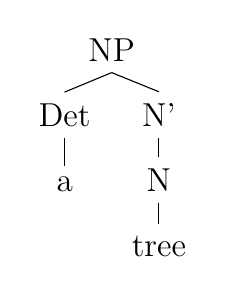
\begin{tikzpicture}
    \Tree
    [.NP
	    [.Det a ]
	    [.N'
		    [.N tree ]
	    ]
    ]
\end{tikzpicture}
\caption{This is a figure made with \code{tikz}}
\label{firsttree}
\end{figure}

Images as figures can be done with the \code{graphicsx} package. The following is a png image showing a syntax tree.

\begin{figure}[htpb!]
    \centering
    \includegraphics[width=6em]{fig}
    \caption{This is an image file}
\end{figure}

When using images for figures, be sure to set the width of the figure to an appropriate value. The source image should also be high enough resolution that it does not look blurry when added to the document.

Complex figures such as pitch contour diagrams may require additional packages. If such are needed, please contact the editors in order to make the necessary arrangements.

\section{Glossing}

Glossing is handled with the \code{linguex} and \code{cgloss} packages. Abbreviations should be lowercase and contained in a \code{\textbackslash textsc\{\}} tag for small capital letters. The following is from van Dam (\citeyear{vandam2019syntax})

\exg.   kaʔ\textsubscript{4} ko\textsubscript{2} nɤ\textsubscript{2} tə\textsubscript{0}-no\textsubscript{1} ʃɯu\textsubscript{1}\\
    down towards {\textsc{prep}} {\textsc{caus}}-extend.horiz {\textsc{imp}} \\~\\
    `point [something] downwards' \label{exg}

References to examples/glossing are handled in the same way as figures, for example here referring to Example \ref{exg} above. The \code{\textbackslash label\{\}} tag can be placed on any line of the example.

\section{Conclusion}

After your conclusion, first list abbreviations (if any), and then references. Consult the references for the type of reference you need, e.g., a book \autocite{anderson2007munda}; a paper in a proceedings publication \autocite{delancey2002bodic}; a journal article \autocites{haokip2012thadou, peterson1998lai}; an unpublished manuscript \autocite{hyslop2010kurtop}; a dissertation \autocite{hyslop2011kurtop}; an edited volume \autocite{morey2008neil}; a chapter in an edited volume \autocite{peterson2003lai}; a conference presentation \autocite{post2008tani}; or a website \autocite{sadokpam2008meetei}.

Abbreviations are organised in a table environment to maintain spacing:

\section*{Abbreviations}

% For each abbreviation, you can use the \abbreviation{}{} tag:

\abbreviation{caus}{Causative prefix}
\abbreviation{imp}{Imperative marker}
\abbreviation{prep}{Preposition}

\listabbreviations

% Do not change anything below this line


% DO NOT CHANGE THIS FILE.

% This file contains all the formatting information required
% to make your document fit the necessary style requirements.
% Any changes you make to this file will be over-written at
% the time of submission. If for any reason you feel it is
% necessary to make changes to this, such as a missing package,
% please contact the editors of North East Indian Linguistics
% to discuss the suggested changes.

% DO NOT MAKE ANY CHANGES WITHOUT APPROVAL FROM THE EDITORS.

\xpatchbibmacro{date+extrayear}{
  \printtext[parens]%
}{
  \setunit{\addperiod\space}
  \printtext
}{}{}

\printbibliography

\end{document}
